\chapter{Overview}
\label{chap:MaxData}
\section{Motivation}
Neuronal models of reinforcement learning assume interactions of midbrain dopaminergic neurons and striatum to compute the differences between anticipated and received outcomes. The nature of this cross-areal interaction is however not fully understood. On this purpose we present an application of the cell-assembly algorithm, at level of pairs, on electrophysiological data from mice.
Dual side in-vivo recordings of electrophysiological activity from Ventral Striatum, including Pallidum, (VS) and Ventral Tegmental Area (VTA), allowed us to study directionality between the two regions.
The novel statistical approach presented treats the temporal scale and precision of coherent activity patterns as free parameters, to be determined from the data, thus, instead to make assumption, we deduced from data temporal scales and precision involved in assemblies pairs with units either from both regions or from only one of the two regions, shedding light on VS-VTA interaction temporal structure and VS-VTA directionality.
We can use the term directionality in our case because we use the algorithm at level of inter-regional pairs. It is important to recall that the cell-assembly algorithm returns lags between the units activation in assembly, thus using the algorithm at level of inter-regional pairs provides us the lag between two units activation, of those two units one is in VS and another in VTA, a lag in activation of such kind of pair, indicates which region is preceding the other in activation.
Our nomenclature was such that a positive lag means that VS is prior in activation, a negative lag, vice-versa, means that VTA is preceding the activation of VS.
Taking advantage of well defined neuron typologies classifications both in VS and VTA, we further investigated the specific cell-type composition of the assemblies exhibiting directionality. 
{\color{red}da finire}
%Using the bin size distribution
\section{State of the art}
 In recent decades Ventral Striatum and Ventral Tegmental area have been widely studied by scientists because of their prediction coding feature.
 To introduce the study on VS-VTA interaction an overview on the state of the art of the Ventral Striatum and Ventral Tegmental area knowledge is needed.
\chapter{Description of experiment and data set}
In this chapter I describe the task and the data collected in our lab.
The task presented is a go/no-go reversal odor discrimination task. Two odors were presented to the mouse, one rewarded (CS+) with reward probability 0.9, the second one unrewarded (CS-). Learning the task consisted in licking at least a defined number of times (two or three depending on the paradigm) during a specific interval, called lick window, when the rewarded odor (CS+) was presented (hit trials) and not licking when unrewarded odor (CS-) was presented (correct rejection trials). Whereas a bad performance consisted in not licking, or licking outside the lick window period, at CS+ presentation (miss trials), or licking at CS- presentation (false alarm trials). Once the performance criterion was reached, the contingencies were switched, in other words the rewarded odor became unrewarded and vice-versa. Once the performance criterion was reached in the reversal phase the extinction phase followed, in which neither one of the two odors was rewarded. The lick window was open for an interval ranging from 1500 $ms$ to 2000 $ms$ depending of different paradigms. after a delay from 500 $ms$ to 1500 $ms$. Only licks happening in the lick window interval were counted as valid to get the reward.
\begin{figure}
    \centering
    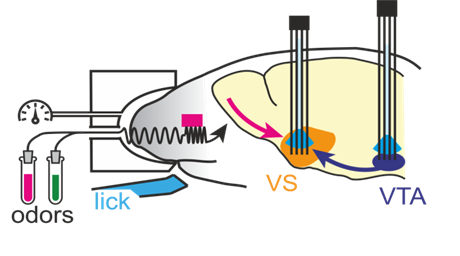
\includegraphics[scale=0.7]{figures/Experiment.png}
    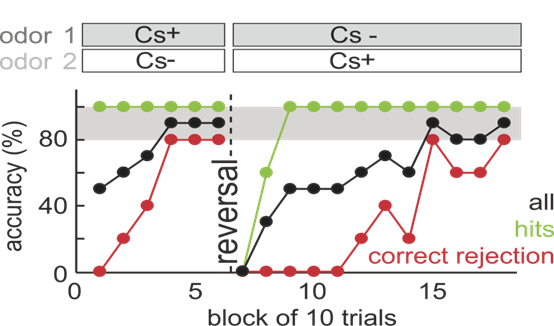
\includegraphics[scale=0.7]{figures/Performance.png}
    \caption{Experimental setup and mice performance}
    \label{fig:experiment}
\end{figure}
\chapter{Single cells analysis}
In this chapter I present the analysis performed on single cells, before to apply the cell-assembly algorithm to the data set.
The principal interest of the project was to investigate the nature of Ventral Striatum and Ventral Tegmental Area. Furthermore it is well known that in both regions different units types are present, a schematic illustration of the brain-circuit of interest is shown in figure(\ref{fig:Brain}).
\begin{figure}
    \centering
    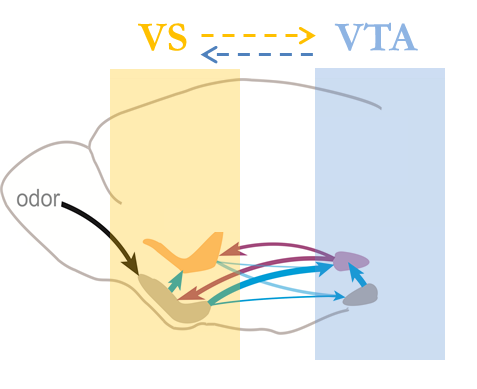
\includegraphics[width=0.45\textwidth]{BrainVSVTA.png}
    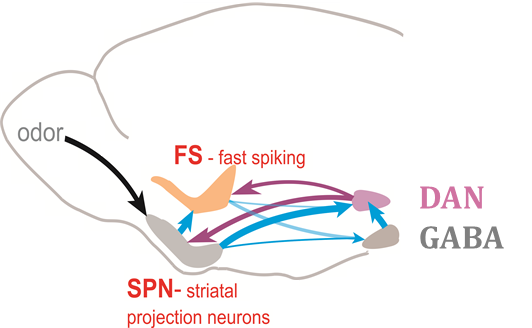
\includegraphics[width=0.45\textwidth]{Brain.png}
    \caption{Caption}
    \label{fig:Brain}
\end{figure}
The circuit effect of interactions makes the nature of themselves puzzling, to figure out which interactions are specifically involved in Reward Prediction and Reward Prediction error, it was matter of interest to understand whether inter-regional interactions between specific cell types have specific characteristics, not found in other cell types.
The data-set included $803$ VS units and $272$ VTA units in total, that were classified in sub-typologies, specifically VS units were classified as either striatal projection neurons (SPNs), fast-spiking neurons (FSNs) or cholinergic interneurons(CINs), according to their firing pattern characteristics computed using only spikes during the inter-trials interval and after session. Units with a firing rate higher than $12 Hz$ were assigned as FSNs and all units with a firing rate below $2 Hz$ as SPNs. Units in the remaining range were designed as putative regular-firing CINs if the CV or their $ISI$ distribution was less than $1.2$ and ISIs less than $60 ms$ contributed no more than $20\%$ of all ISIs. Finally the resting units were characterized as SPNs or FSNs if they ever were silent for more than $2 s$. Using this classification mean normalized autocorrelations and mean waveforms have canonical patterns. It is important to make a clarification about FSN: it can be assumed that the recorded FSNs are pallidal neurons, in fact FSNs in Striatum represent only $<5\%$ of the population({\color{red}ask for a paper to cite}), while pallidal units have higher firing rate ({\color{red} sk for a paper to cite}). %(\ref{fig:AutoVS}).
VTA units were instead classified as Dopaminergic neurons (DAN), Gabaergic units (GABA), and Cholinergic interneurons (CHI) according to their task related activity using a clustering approach adapted from (\cite{Uchida}). First, response were characterized for the relevant time spans ({\color{red}ask Max for the updated intervals}(CS+ from 0 to 0.5 and US from -0.5 to 0 and from 0 to 0.5), significant task related response were assessed with Friedman test, and only significant units ($p<0.05$) were included in the clustering classification.{\color{red}part of classification has to be included}
%\begin{figure}
%  \centering
 %   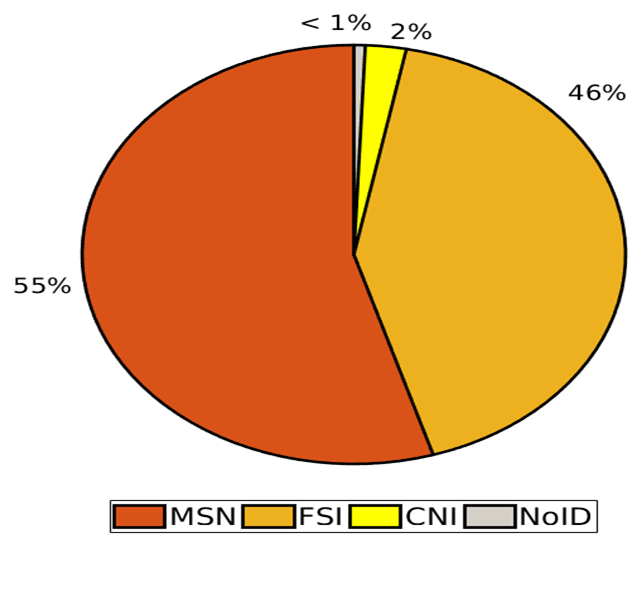
\includegraphics[scale=0.5]{figures/PieRegVS.png}
  %  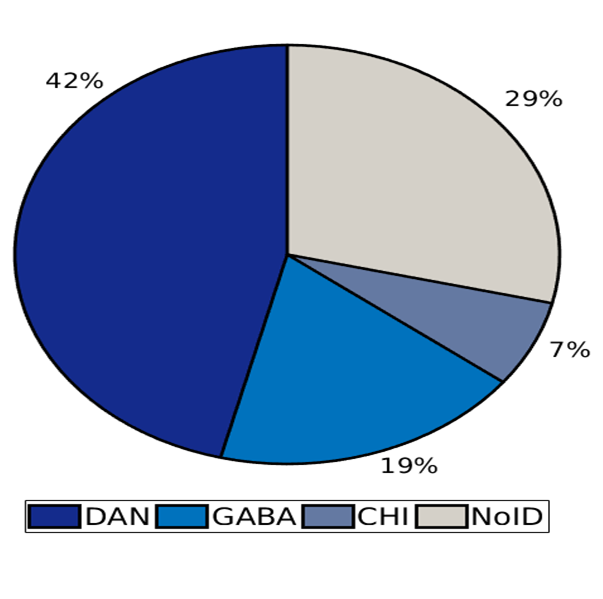
\includegraphics[scale=0.5]{figures/PieRegVTA.png}
   %\caption{Caption}
   % \label{fig:PieRegions}
%\end{figure}

\begin{figure}
  \centering
    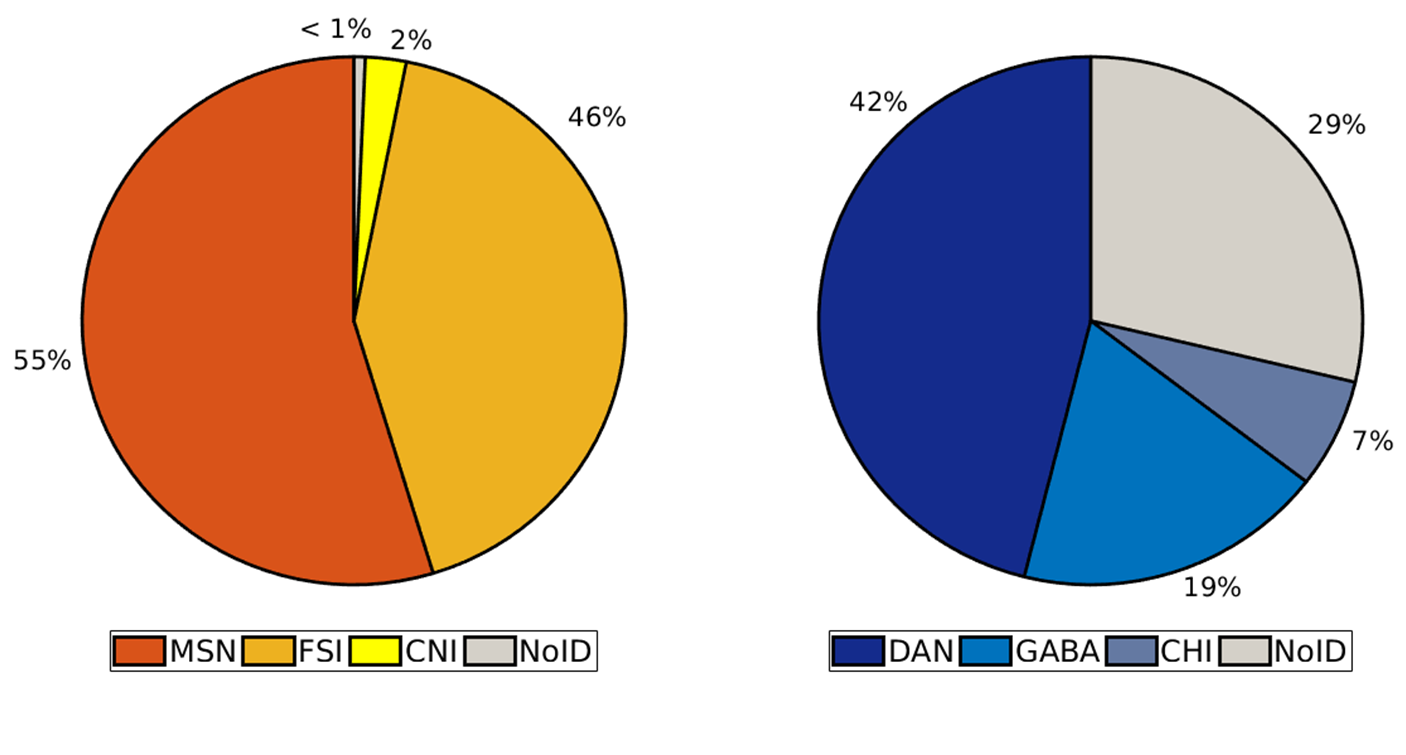
\includegraphics[scale=0.6]{figures/PieGroup.png}
   \caption{Caption}
    \label{fig:PieRegions}
\end{figure}
%\begin{figure}
 %   \centering
  %  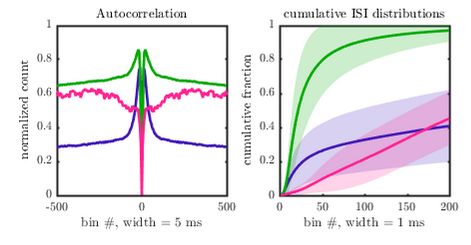
\includegraphics[scale=0.7]{figures/AutocorrelationVSunits.png}
   % \caption{Caption}
    %\label{fig:AutoVS}
%\end{figure}({\color{red}citation of graybiel 2005 if it is the rigth paper})
%distributed as shown in fig.(\ref{fig:GlobalPie})
